\documentclass[a4paper,11pt,german]{scrartcl}

\usepackage[T1]{fontenc}
\usepackage[utf8]{inputenc}
\usepackage[ngerman]{babel}
\usepackage[left=20mm, right=20mm, top=25mm, bottom=60mm]{geometry}
\usepackage{graphicx}
\usepackage{listings}

\newcommand{\email}{\large{\texttt{\{vdittmer\}@edu.aau.at}}}
\title{Key-Frame-based Video Browser with HTML5}
\subject{Fundamental Topics in Distributed Multimedia Systems}
\author{Mario Graf, Verena Dittmer, Jameson Steiner}

\providecommand{\tightlist}{%
  \setlength{\itemsep}{0pt}\setlength{\parskip}{0pt}}

\begin{document}

\maketitle

\section*{Implementierung}
Wir haben uns für die Umsetzung dazu entschieden, die Applikation rein unter Verwendung des Canvas-Elements zu implementieren. Dadurch wirkt der Quellcode der \lstinline$index.html$ Datei sehr übersichtlich und aufgeräumt:

\begin{verbatim}
<body>
<div id="container">
  <video width="854" height="480" id="videoElement">
    <source src="media/bunny.mp4" type="video/mp4">
    Your browser does not support HTML5 video.
  </video>
  <canvas id="keyframeBrowser" width="854" height="100"></canvas>
  <canvas id="timeline"></canvas>
  <div id="controls">
    <button type="button" id="play-pause" class="play">Play/Pause</button>
    <input type="range" id="volume-bar" min="0" max="1" step="0.1" value="1">
  </div>
</div>
</body>
\end{verbatim}

Es werden zwei Canvas Elemente eingesetzt:
\begin{itemize}
\tightlist
\item \textbf{keyFrameBrowser: } Wird verwendet um die Thumbnails und deren Animationen zu rendern. Die Implementierung dazu befindet sich in \textbf{KeyframeBrowser.js}.
\item \textbf{timeline: } Wird verwendet um die dazugehörige Timeline zu rendern. Die Implementierung dazu befindet sich in \textbf{timeline/Timeline.js}.
\end{itemize}

\begin{figure}[ht!]
	\centering
  	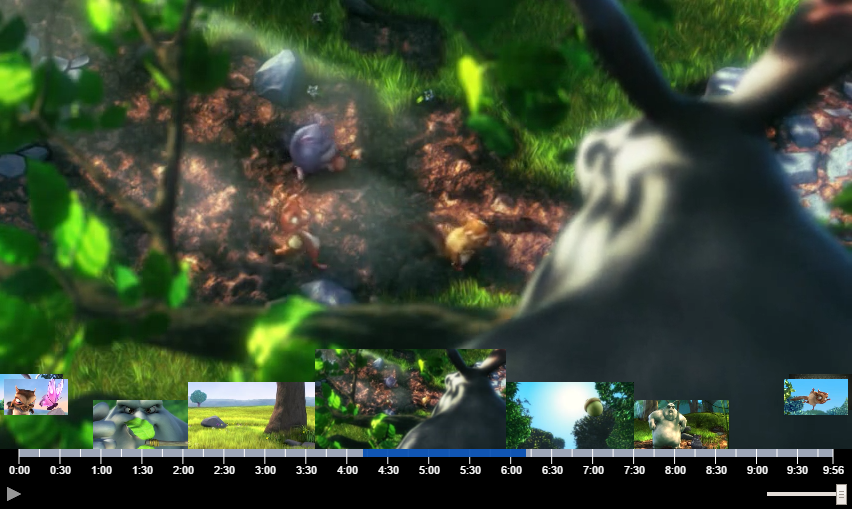
\includegraphics[width=0.7\textwidth]{images/videoBrowserZoomIn.png}
	\caption{Die 5 Keyframes und die Stapel der Nachbarclusters des zweiten Levels}
	\label{zoomedIn}
\end{figure}

Eine lauffähige Version dieses Projektes kann unter \lstinline$www.jmsn.at/videoBrowser$ ausprobiert werden. Wir haben unsere Implementierung unter Chrome und Safari getestet.

\section*{Keyframes- und Segment-Generierung}
Als Testvideo für unseren Player haben wir Big Buck Bunny verwendet. Hierfür wurden die Thumbnails mittels ffmpeg extrahiert. Alle 5 Sekunden wird dabei ein Keyframe mit reduzierter Auflösung erstellt.

Aus den Thumbnails wird mittels dem \texttt{Clustering} Java-Programm (zu finden im Ordner \lstinline$clustering$) ein Json-File erstellt, welches die unterschiedlichen Level der Segmente anzeigt. In dem Json-File steht für jeden Keyframe der Dateiname, die \texttt{FromTime} und \texttt{ToTime} (d.h die früheste und späteste Zeit von allen Frames der Level drunter), die Abspielzeit in Sekunden im Video, und die jeweiligen Keyframes von einem Level drunter. Das mittlerste Keyframe ist dabei der Repräsentant für ein Level darüber.

\section*{Darstellung der Thumbnails}
Um die zahlreichen Animationen der darzustellenden Thumbnails bewerkstelligen zu können, haben wir eine eigene Render- und Animationsengine implementiert (\textbf{RenderingEngine.js}). Diese Engine hält eine Referenz zu allen dargestellten Thumbnails. Jedes Thumbnail ist eine Instanz von \lstinline$Renderable$ (\textbf{Renderable.js}) und liefert die nötigen Informationen für die Berechnung der Animation.

Die Engine ist in der Lage Position, Größe (Skalierungsfaktor) und Transparenz der einzelnen Renderables zu animieren.

Besonders herausfordernd war dabei, die Animationen und Übergänge zwischen den Hierachien derart zu gestalten, dass der Benutzer auch versteht bzw. einen Eindruck davon bekommt was gerade durch seine Mausinteraktion passiert (zoom-in Effekt, side-scroll Effekt).

\section*{Timeline}
Die Timeline kann parametrisiert über die Videolänge und die gewünschte Breite der Timeline erstellt werden. Hierfür werden innerhalb eines Canvas der blaue Hintergrundstreifen, die Timestamps und die zugehörigen Striche in entsprechenden Abständen generiert. Eine weitere Funktion bietet die Möglichkeit, einen bestimmten Bereich des Videos einzufärben. Dies wird für das Anzeigen der Positionen der Keyframes innerhalb des Videos genutzt. Hierfür wird die \texttt{FromTime} des linkesten und die \texttt{ToTime} des rechtesten Keyframes der Timeline zum Einfärben übergeben. 

\section*{Abspielen des Videos}
Durch Klicken auf einen Keyframe wird das Video ab dieser Stelle abgespielt. Hierfür wird die Abspielzeit, die im Json-File zu dem zugehörigen Keyframe gespeichert war, dem Video zum Abspielen übergeben.


\end{document}
